\section{El contexto de la ingeniería de software}
Un modelo de proceso de software se utiliza para describir los pasos a seguir y las actividades a realizar cuando se desarrolla software. Algunos ejemplos de modelos de proceso de software son el modelo cascada, el desarrollo incremental, el desarrollo evolucionario y el modelo espiral.

En la figura debe notarse que el proceso es esencial, ya sea si se trabaja en el desarrollo de un nuevo producto o si se está manteniendo uno existente.

\begin{figure}[H]
\centering
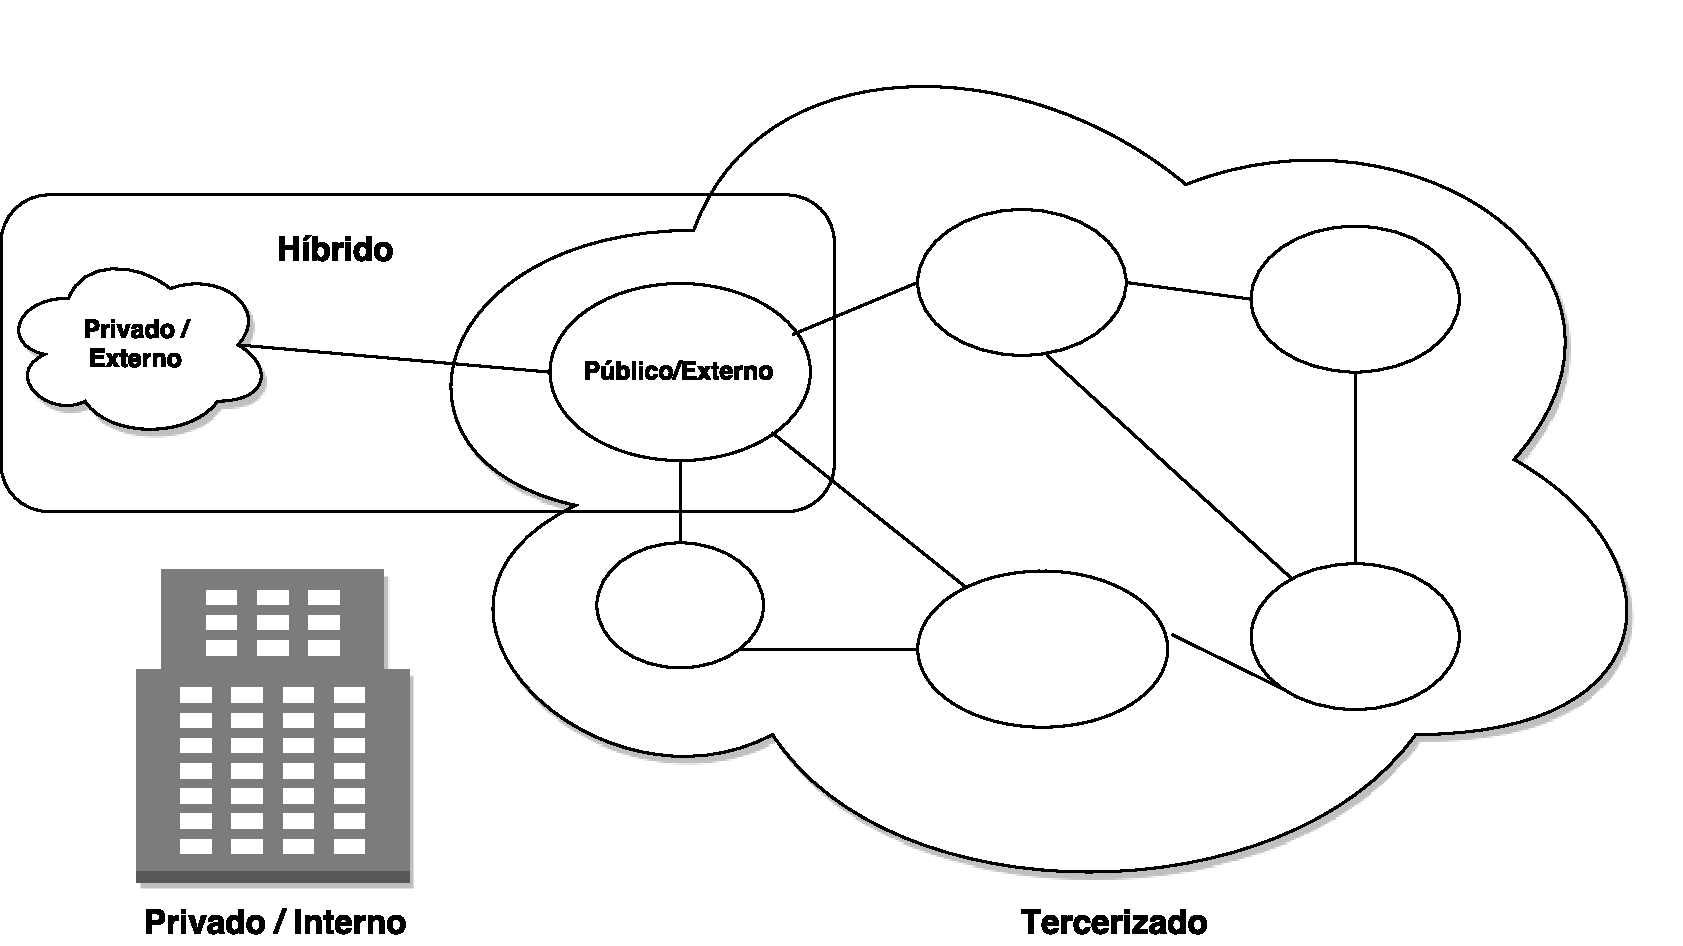
\includegraphics[width=125mm,scale=1]{Figuras/cloud_computing_types}
\caption{HACER MI PROPIO DIAGRAMA.}
  \label{software_process}
\end{figure}